\section{Critical Years (15K,12P)}

Following are the critical point with respect to the Lots, especially if malefics are in conjunction or in aspect with Fortune\footnote{Robert Hand points out the years with respect to Fortune are ``clearly derived from profections through the houses'' while the \textsl{Critical Years} of the signs are derived from one of the sign's triplicity rulers although he says it is not clear why one is chosen over another (VRS3 71). Bracketed, italicized numbers are those given in VRS3 p70-1.}
:
\footnotesize
\begin{center}
\begin{tabular}{lS}
\toprule
\textbf{Position of Malefic} & 
	\textbf{Every \textit{n} Years}\\
\midrule
in \Opposition & 7 \\
\Trine\xspace on the right & 9 \\
\Trine\xspace on the left & 5 \\
\Square\xspace on the right & 10 \\
\Square\xspace on the left & 4 \\
\Sextile\xspace on the right & 11 \\
\Sextile\xspace on the left & 3 \\
in the sign preceding the Lot & 12 \\
in contact with the Lot & 2 \\
\bottomrule
\end{tabular}

\begin{tabular}{cS}
\toprule
\textbf{Position of \Fortune} & 
	\textbf{Every \textit{n} Critical Years} \\
\midrule
\Aries\xspace & \textsl{[19]} \\
\Taurus\xspace & \textsl{[25]} \\
\Gemini\xspace & 20 \\
\Cancer\xspace & 25 \\
\Leo\xspace & 12 \\
\Virgo\xspace & 8 \\
\Libra\xspace & 30 \\
\Scorpio\xspace & 15 \\
\Sagittarius\xspace & 12 \\
\Capricorn\xspace & 8 \\
\Aquarius\xspace & 30 \\
\Pisces\xspace & 15 \\
\bottomrule
\end{tabular}
\end{center}
\normalsize
\textbf{/157K/}

\subsection{The Mean Years of the Stars (15K,13P)}

Following are the mean years of the stars\footnote{See comment and table on next page.}:
\begin{table}[ht]
\begin{center}
\label{Table 3.1}
\begin{tabular}{lS}
\toprule
\textbf{Planet} & \textbf{Years} \\
\midrule
\Saturn & 45 \\
\Jupiter & 49 \\
\Mars & 42 \\
\Venus & 46 \\
\Mercury & 48 \\
\Sun & 64 \\
\Moon & 67 \\
\bottomrule
\end{tabular}
\caption{Mean Years of the Stars}
\end{center}
\end{table}

The stars allot \textbf{/149P/} these years plus their periods or the rising times of their signs whenever they happen to be operative.

Another system of mean years: you will find the mean years by adding the maximum and the minimum periods. For example: the complete period of \Saturn\xspace is 57 years and the minimum is 30, for a total of 87, half of which is 43 1/2.  The complete period of \Jupiter\xspace is 79 and the minimum is 12, for a total of 91, half of which is 45 1/2. And so on for the rest of the stars.

Now the rising times of the signs in the Tables of Rising Times of Hypsicles are in error if the period <in question> amounts to one or two years \ldots but the King has revealed the rising times only for the first klima.

\begin{mdframed}[backgroundcolor=cyan!5]
\textbf{Comment:} \hfill \\
As Robert Hand mentions in the VRS3 translation, the planet years, as shown above table, are not as given in the majority of sources, but rather as Valens mentions them in the examples below. For reference, here is a table of Planet Years as they are usually given:
\end{mdframed}

\begin{table}[ht]
\begin{center}
\label{Table 3.3}
\aboverulesep=0pt
\belowrulesep=0pt
\begin{tabular}{|c c c c|}
\toprule
\rowcolor{cyan!5} 
	\textbf{Planet} & \textbf{Minor}
                      & \textbf{Medium} & \textbf{Major} \\
\midrule
\rowcolor{cyan!5}  \Saturn & 30 & 43.5 & 57 \\
\rowcolor{cyan!5}  \Jupiter & 12 & 45.5 & 79 \\
\rowcolor{cyan!5}  \Mars & 15 & 40.5 & 66 \\
\rowcolor{cyan!5}  \Venus & 8 & 45 & 82 \\
\rowcolor{cyan!5}  \Mercury & 20 & 48 & 76 \\
\rowcolor{cyan!5}  \Sun & 19 & 69.5 & 120 \\
\rowcolor{cyan!5}  \Moon & 25 & 66.5 & 108 \\
\bottomrule
\end{tabular}
\caption{Years of the Planets (as usually given)}
\end{center}
\end{table}

\newpage
An example: \Sun, \Venus, \Mercury\xspace in \Cancer, \Moon\xspace in \Taurus, \Saturn in \Pisces, \Jupiter, \Mars\xspace in \Leo, Ascendant in \Virgo 
\footnote{\textit{Greek Horoscopes} dates the chart (L82) to approximately July 9, 82 AD(p.92). This is actually Chart 7 from Book II, section 21, with some differences (errors) in the placement of the Ascendant and \Venus. Robert Hand, in a footnote to the chart in Schmidt's version, says the errors do not affect the methodology being described (VRS3 p.72).}.

\clearpage
\begin{wrapfigure}[14]{R}{7cm}
\centering
\vspace{-20pt}
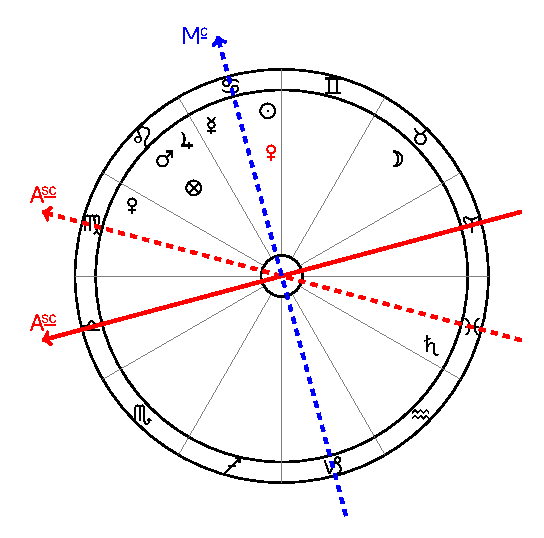
\includegraphics[width=0.68\textwidth]{charts/3_15_1}
\caption{Chart 7a [III.15.1, GH L82]}
\label{fig:chart7a}
\end{wrapfigure} 

In the first klima the rising time of \Virgo\xspace is 38 1/3. Since \Mercury,the ruler <of \Virgo>, is in \Cancer, in <the XI Place of the> Good Daimon, it contributed its rising time, 31 2/3. The total is 70; the native lived that long.

\newpage
Another example: \Sun, \Mercury\xspace in \Taurus, \Moon\xspace in \Pisces, \Saturn\xspace in \Scorpio, \Jupiter, \Mars, \Venus in \Aries, Ascendant in \Gemini
\footnote{\textit{Greek Horoscopes} dates the chart (L102,IV,a) to approximately April 30, 102 AD(p.100)}.

\clearpage
\begin{wrapfigure}[9]{R}{7cm}
\centering
\vspace{-20pt}
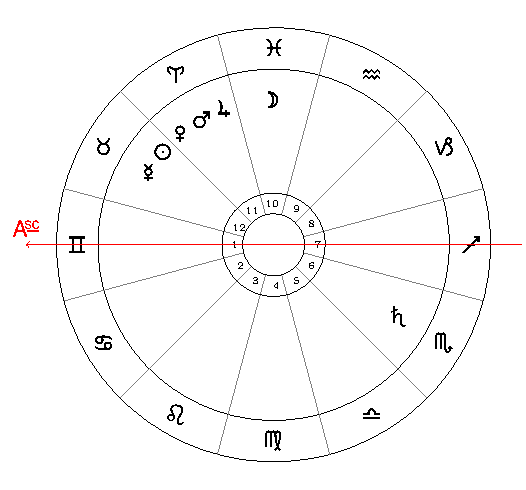
\includegraphics[width=0.68\textwidth]{charts/3_15_2}
\caption{Chart 50 [III.15.2, GH L102, IV, a]}
\label{fig:chart50}
\end{wrapfigure} 

The rising time <of \Gemini> in the second klima is 28. \Mercury\xspace in \Taurus\xspace adds its rising time, 24, plus \Mars\xspace and \Venus\xspace in \Aries, 15. He died in his 67th year\footnote{Robert Hand notes that the timing is from \Gemini's ascension time (28°) + its ruler \Mercury\, in \Taurus\, giving \Taurus's rising time (24°) + \Mars's minor years (15°) as it rules \Venus, ruler of \Taurus, posited in \Aries\, and ruled by \Mars\, for a sum total of (28 + 24 + 15) 67 years (VRS3 p72).}.

\newpage
Another example: the same configuration of stars <as in the preceding horoscope> for a different nativity, except that the Ascendant was in \Capricorn, the Lot of Fortune in \Pisces
\footnote{\textit{Greek Horoscopes} dates the chart (L102,IV,b) to approximately April 30, 102 AD(p.100)}.

\clearpage
\begin{wrapfigure}[11]{R}{7cm}
\centering
\vspace{-28pt}
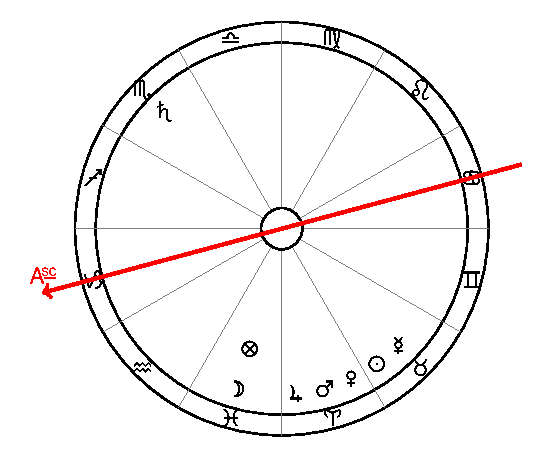
\includegraphics[width=0.68\textwidth]{charts/3_15_3}
\caption{Chart 51 [III.15.3, GH L102,IV, b]}
\label{fig:chart51}
\end{wrapfigure} 

The rising time <of \Pisces> in the second klima is 20, plus the period of \Jupiter, 12. Since \Jupiter\, is in \Aries, we add its \textsl{[\Aries]} rising time, 20, plus the period of \Mars, 15. The total is 67. He lived that long. \\
\newline
\newline
These chapters which I have composed may seem unprofessional because they have been addressed to a youthful audience, my students, in such a way that they might find my introduction to this art comprehensible. In view of this fact, I had wished to revise them for greater accuracy, but I have not had the opportunity because my vision has been troubled and my intellectual capacity has been enfeebled by my deep sorrow for a precious student who has died. May the reader pardon me.

End of the\textit{Anthologies} of Vettius Valens of Antioch, Book III.

\newpage